\section{Autómata finito determinista}\label{FiniteAutomaton}
Formalmente, un autómata finito es una 5-tupla ($Q, \Sigma, q_{0}, \delta, F$) donde:

\begin{itemize}
	\item $Q$, es un conjunto finito de estados;
	\item $\Sigma$, es un conjunto finito de \glspl{symbol} llamado \gls{alphabet};
	\item $q_{0}\in Q$ es el estado inicial;
	\item $\delta \colon Q\times \Sigma \to Q$ es una función de transición;
	\item $F\subseteq Q$ es un conjunto de estados finales o de aceptación.
\end{itemize}

Un \acrfull{AFD}, es un autómata/máquina que tiene un número finito de estados y además es un sistema determinista, es decir, para cada \gls{symbol} de entrada, se puede determinar el estado al que se moverá el autómata \cite{wiki:Automata_finito}. 

Un \acrshort{AFD} está representado por un grafo dirigido llamado diagrama de estado.

\begin{itemize}
	\item Los estados son representados por vértices o nodos $Q = \{ S_1, S_2, S_3, \dots \}$.
	\item Las aristas o arcos etiquetados con un \gls{alphabet} $\Sigma$, representan las transiciones $\delta$.
	\item El estado inicial $q_{0}$ se denota por una sola arista entrante vacía.
	\item El o los estados finales $F$ están indicados por círculos dobles.
	\item Cada transición se escribe  $\delta ( q_1, \sigma ) = q_2$,  también se puede denotar como $q_1 \xrightarrow{\sigma} q_2$.
\end{itemize}

\subsection{Ejemplo}
El siguiente ejemplo es de un \acrshort{AFD} $L$, con un alfabeto binario, que reconoce el lenguaje regular conformado exclusivamente por las cadenas con un número par de ceros y un número par de unos.

$M = (Q, \Sigma, q_{0}, \delta, F)$ donde:
\begin{itemize}
	\item $Q = \{S_1, S_2, S_3, S_4 \}$
	\item $\Sigma = \{ 0, 1 \}$
	\item $q_0 = S_1$
	\item $F = \{ S1 \}$
	\item $\delta:  
			\delta(S_1, 0) = S_3, 
			\delta(S_1, 1) = S_2,
			\delta(S_2, 0) = S_4,
			\delta(S_2, 1) = S_1,
			\delta(S_3, 0) = S_1,
			\delta(S_3, 1) = S_4,
			\delta(S_4, 0) = S_2,
			\delta(S_4, 1) = S_3
		$
\end{itemize}

\begin{figure}[H]
	\centering
	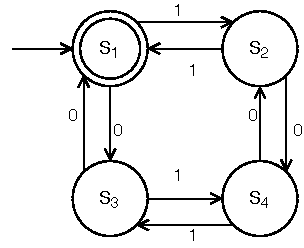
\includegraphics[width=0.4\linewidth]{doc/FiniteAutomaton/img/AFD}
	\caption{El diagrama de estado de $L$}
	\label{fig:AFD}
\end{figure}

El lenguaje reconocido por $L$ es el lenguaje regular dado por la expresión regular \cite{stackoverflow:Biegeleisen2015}: 
$$
^\wedge(00|11|(01|10)(00|11)^\ast(01|10))^\ast \$
$$

La Figura \ref{fig:AFD} da un ejemplo de un autómata simple $M$ que acepta la cadena:
$$
1001101011001010010001
$$

% https://en.wikipedia.org/wiki/Deterministic_finite_automaton
% https://es.wikipedia.org/wiki/Teor%C3%ADa_de_aut%C3%B3matas
